\documentclass[11pt,a4paper]{ctexart}
\usepackage{geometry}
\geometry{margin=2.2cm}
\usepackage{graphicx}
\usepackage{booktabs}
\usepackage{xcolor}
\usepackage{float}
\usepackage{caption}
\usepackage{array}
\usepackage{enumitem}
\usepackage{fancyhdr}
\definecolor{accent}{HTML}{2563EB}
\captionsetup{font=small,labelfont=bf}
\pagestyle{fancy}\fancyhf{}
\lhead{ResumAI Agent 端到端压测报告}\rhead{\thepage}
\renewcommand{\headrulewidth}{0.4pt}

\title{\textbf{ResumAI Agent 系统\\100 份简历端到端压测报告}}
\author{自动化压测 Harness · 阿里云 ECS 真实采集}
\date{生成时间：2026-06-26T10:57:30}

\begin{document}
\maketitle
\thispagestyle{fancy}

\begin{abstract}
本报告对部署于阿里云 ECS（后端 base \texttt{http://8.138.10.189}）的 ResumAI Agent 简历评估系统，
执行了 \textbf{100 份简历}的真实端到端压测。采集方式为纯 HTTP 调用（\texttt{curl.exe} 上传 + 轮询任务状态 +
拉取 agent-execution 全链路 trace），并发上限 4，逐份解析 LangGraph DAG 各节点时延、工具调用、
动态路由计划与评分结论。\textbf{成功 100/100（成功率 100.0\%，失败率 0.0\%）}。
端到端处理时延 \textbf{p50=38.5s / p90=48.5s / p95=51.3s（均值 38.6s，max 55.7s）}；
动态路由共出现 \textbf{4 种 routeMode}，相比固定全量流水线累计节省 \textbf{93 次大模型调用}
（607/700，节省 13.3\%）；
公网 MCP fetch 触发率 70.0\%（70/100），与简历清单中含 GitHub/外链比例 70.0\%（70/100）高度吻合，公网 MCP 平均时延 \textbf{3.15s}。
所有数据均为真实采集，未做任何编造。
\end{abstract}

\section{压测方法}
\begin{itemize}[leftmargin=1.4em]
  \item \textbf{数据集}：\texttt{testdata/stress\_resumes/} 共 100 份简历（PDF/TXT 混合，覆盖资深后端、AI Agent、
  大模型应用、前端、产品、数据平台、SRE、算法、测试、安全、移动端、应届、职业空窗、稀疏风险等 15 类角色），
  清单 \texttt{manifest.json} 提供 id/role/fileType/hasGithub/textLength/expectedSkills 等元数据。
  \item \textbf{提交}：对每份简历用 \texttt{curl.exe -F "file=@<path>;type=..." -F "executionMode=DAG\_CONCURRENT"}
  调用 \texttt{POST /api/tasks/upload-auto}（subprocess 直接调用，规避 PowerShell 转义），解析返回的 \texttt{traceId}。
  \item \textbf{并发与轮询}：最多同时 in-flight 4 个任务，提交后每 5s 轮询 \texttt{GET /api/tasks/\{traceId\}}
  直至 \texttt{status} 为 \texttt{SUCCESS/FAILED}，单任务超时上限 180s。
  \item \textbf{trace 采集}：成功任务再调 \texttt{GET /api/tasks/\{traceId\}/agent-execution}，解析每个 DAG 节点的
  \texttt{durationMs}、全部 \texttt{toolCalls}（name/durationMs/status）、内嵌的 \texttt{harnessPlan}
  （routeMode / selectedAgents / estimatedLlmCalls / llmCallsSavedVsFull）以及任务级 score/recommendation/
  报告正文/面试追问。
  \item \textbf{可复现 \& 断点续跑}：采集脚本 \texttt{harness/run\_stress.py}，每完成一份即落盘 \texttt{checkpoint.json}，
  原始全量结果 \texttt{raw\_results.json}，汇总 \texttt{summary.json}。
\end{itemize}

\section{系统架构简述}
ResumAI Agent 采用 \textbf{LangGraph DAG 编排}的多 Agent 流水线，核心机制：
\begin{itemize}[leftmargin=1.4em]
  \item \textbf{LangGraph DAG}：意图识别 $\to$ 简历解析 $\to$ JD 匹配 $\to$ 知识检索 $\to$（技术/项目/风险评估）$\to$ 证据融合 $\to$ 报告生成。
  \item \textbf{动态路由 Harness}：在 \texttt{knowledge\_context} 阶段构建 \texttt{harnessPlan}，依据简历复杂度/技术信号/项目信号/
  风险信号，动态选择是否启用 \texttt{tech\_eval / project\_eval / risk\_eval} 可选节点，从而\textbf{按需裁剪 DAG、减少大模型调用}。
  \item \textbf{公网 MCP fetch}：通过官方公共 MCP 服务器 \texttt{mcp-server-fetch} 真实抓取候选人外部主页（GitHub/博客），
  工具名 \texttt{mcp\_fetch[public:mcp-server-fetch]}，并在 trace 中可观测其时延。
  \item \textbf{GitHub 富集}：\texttt{github\_enrichment} 在技术评估阶段对带外链的简历做外部证据增强。
  \item \textbf{知识库 RAG}：\texttt{milvus\_resume\_batch\_search / knowledge\_search} 基于向量库注入评分量纲（rubric）证据。
  \item \textbf{分层 Memory}：路由计划中体现 \texttt{memoryHitCount}，复用历史评估记忆影响裁剪与判定。
\end{itemize}

\section{总体结果与端到端时延}
\begin{table}[H]\centering\caption{总体结果}
\begin{tabular}{l r}
\toprule
指标 & 数值 \\
\midrule
简历总数 & 100 \\
成功 / 失败 & 100 / 0 \\
成功率 & 100.0\% \\
失败率 & 0.0\% \\
端到端处理时延 均值 & 38.6 s \\
p50 / p90 / p95 & 38.5 / 48.5 / 51.3 s \\
max / min & 55.7 / 10.7 s \\
客户端墙钟时延 p50/p90（含排队）& 44.1 / 54.9 s \\
\bottomrule
\end{tabular}\end{table}

\begin{figure}[H]
\centering
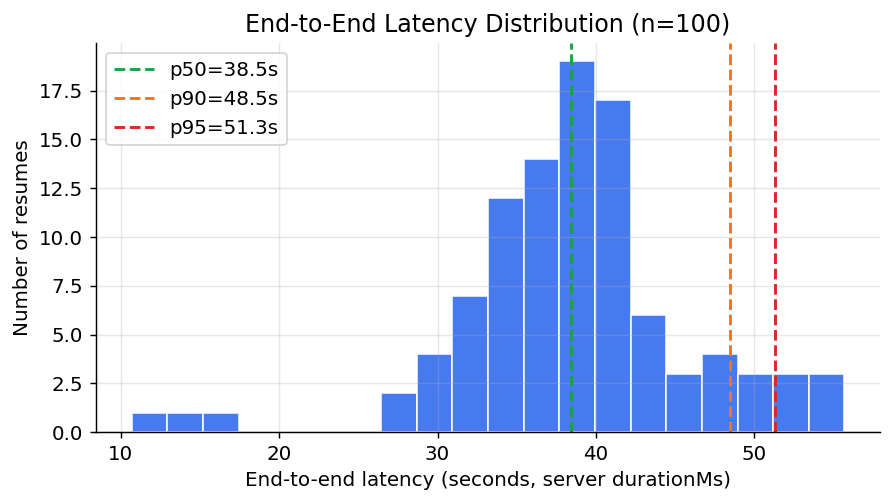
\includegraphics[width=0.86\textwidth]{figs/latency_hist.png}
\caption{端到端处理时延分布（基于任务级 durationMs，标注 p50/p90/p95）}
\end{figure}


\section{各 Agent 节点时延与瓶颈}
下表与图为各 DAG 节点的平均时延（仅统计实际执行该节点的任务）。瓶颈节点为
\textbf{技术评估 TechEvalAgent}，平均 \textbf{13.86s}。
\begin{table}[H]\centering\caption{各节点平均时延}
\begin{tabular}{l r r}
\toprule
节点（Agent） & 平均时延 (s) & 样本数 \\
\midrule
意图识别 IntentAgent & 6.09 & 100 \\
简历解析 ResumeParseAgent & 4.41 & 100 \\
JD 匹配 JdMatchAgent & 3.08 & 100 \\
知识检索+MCP KnowledgeRetrievalAgent & 2.89 & 100 \\
技术评估 TechEvalAgent & 13.86 & 97 \\
项目评估 ProjectEvalAgent & 10.89 & 59 \\
风险评估 RiskAgent & 4.97 & 51 \\
证据融合 EvidenceFusionAgent & 0.11 & 100 \\
报告生成 ReportAgent & 11.93 & 100 \\
\bottomrule
\end{tabular}\end{table}

\begin{figure}[H]
\centering
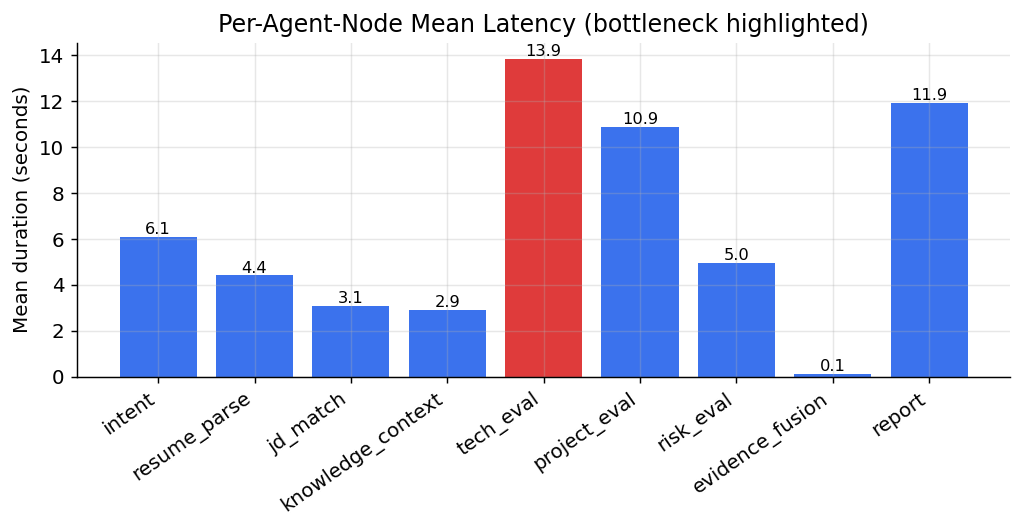
\includegraphics[width=0.86\textwidth]{figs/node_duration_bar.png}
\caption{各 Agent 节点平均时延（红色为瓶颈节点）}
\end{figure}


\section{动态路由分析（证明对不同简历路由不同）}
本次压测共触发 \textbf{4 种 routeMode}，说明系统根据简历内容动态选择评估路径，而非固定流水线。
\begin{table}[H]\centering\caption{routeMode 分布}
\begin{tabular}{l l r r}
\toprule
routeMode & 含义 & 数量 & 占比 \\
\midrule
TECH\_DEEP\_DIVE & 技术深评 & 49 & 49.0\% \\
TECH\_SCREEN & 技术初筛 & 38 & 38.0\% \\
FULL\_REVIEW & 全量评估 & 10 & 10.0\% \\
FAST\_SCREEN & 快速筛选（稀疏简历） & 3 & 3.0\% \\
\bottomrule
\end{tabular}\end{table}

\begin{figure}[H]
\centering
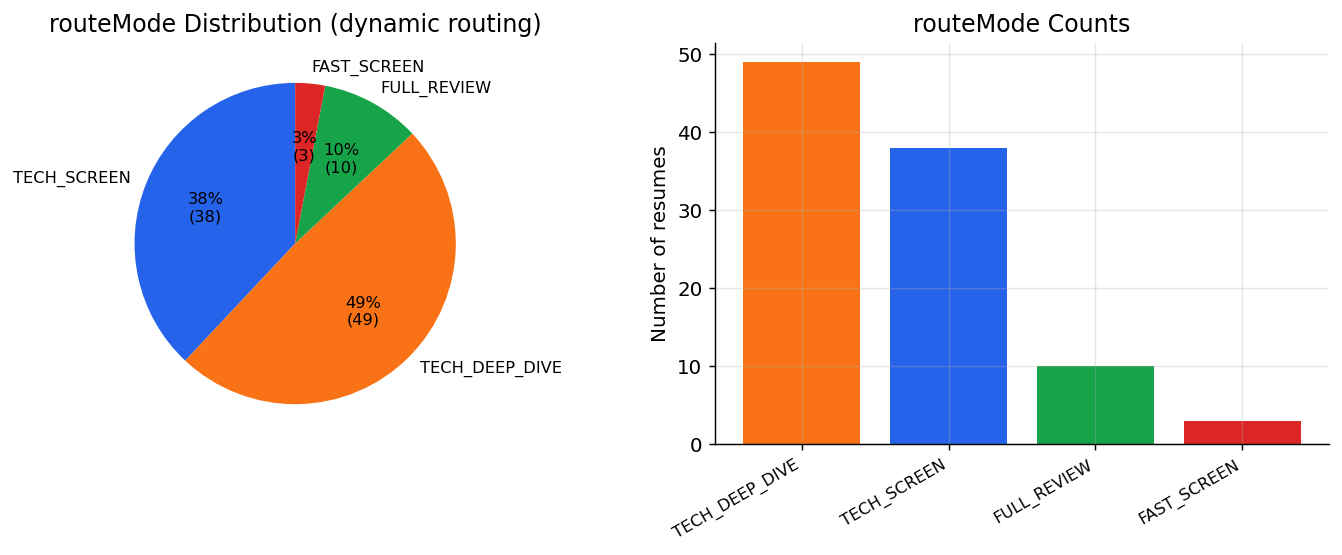
\includegraphics[width=0.86\textwidth]{figs/routemode_dist.png}
\caption{routeMode 分布（饼图 + 柱状）：不同简历走不同评估路径}
\end{figure}


\section{动态路由 / Memory 对大模型调用的节省}
固定全量流水线每份需 7 次 LLM 调用
（intent+resume\_parse+jd\_match+report 固定 4 次，tech/project/risk 可选 3 次；evidence\_fusion 为确定性无 LLM）。
动态路由后每份平均仅 \textbf{6.07} 次。
\textbf{累计节省 93 次（607/700，节省 13.3\%）}。
\begin{table}[H]\centering\caption{每份简历节省的 LLM 调用次数分布}
\begin{tabular}{r r}
\toprule
节省次数/份 & 简历数 \\
\midrule
0 & 10 \\
1 & 87 \\
2 & 3 \\
\bottomrule
\end{tabular}\end{table}

\begin{figure}[H]
\centering
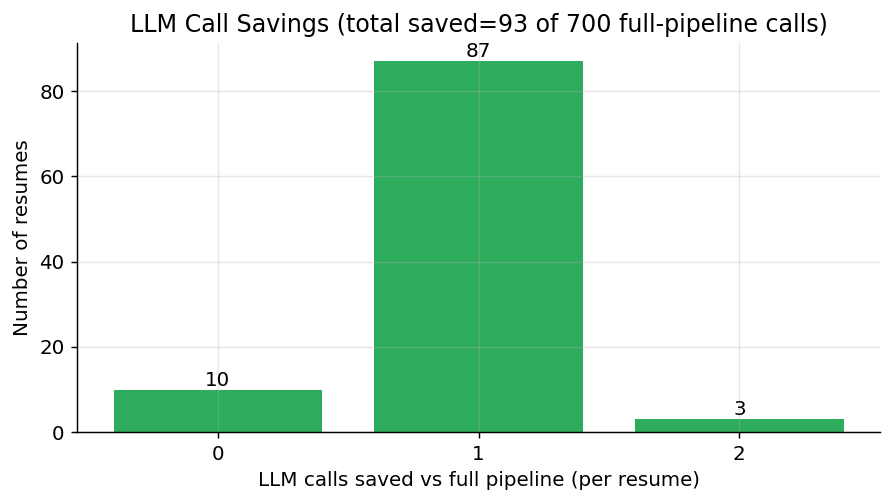
\includegraphics[width=0.86\textwidth]{figs/llm_saved_bar.png}
\caption{LLM 调用节省分布（动态路由 + 分层 Memory 的直接收益）}
\end{figure}


\section{公网 MCP fetch 与 GitHub 富集}
公网 MCP fetch 触发率 70.0\%（70/100），与简历清单中含 GitHub/外链比例 70.0\%（70/100）高度吻合。
\begin{table}[H]\centering\caption{公网 MCP / GitHub 富集统计}
\begin{tabular}{l r}
\toprule
指标 & 数值 \\
\midrule
MCP fetch 触发任务数 & 70 \\
MCP fetch 触发率 & 70.0\% \\
MCP fetch 调用总次数 & 70 \\
MCP fetch 平均时延 & 3.15 s \\
MCP fetch p90 / max 时延 & 3.88 / 5.99 s \\
github\_enrichment 触发率 & 69.0\% \\
github\_enrichment 平均时延 & 0.52 s \\
简历清单含外链比例 & 70.0\% \\
\bottomrule
\end{tabular}\end{table}

\begin{figure}[H]
\centering
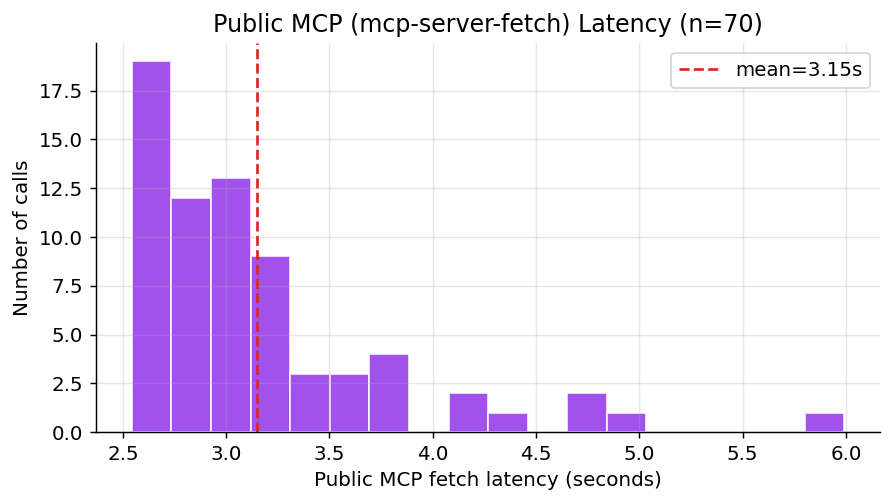
\includegraphics[width=0.86\textwidth]{figs/mcp_latency.png}
\caption{公网 MCP（mcp-server-fetch）真实接入时延分布}
\end{figure}


\section{评分与推荐结论分布}
评分均值 73.6（p50=72.0，max=86.0，min=39.0）。
\begin{table}[H]\centering\caption{推荐结论分布}
\begin{tabular}{l r r}
\toprule
推荐结论 & 数量 & 占比 \\
\midrule
RECOMMEND & 9 & 9.0\% \\
NEED\_MANUAL\_REVIEW & 7 & 7.0\% \\
NOT\_RECOMMEND & 84 & 84.0\% \\
\bottomrule
\end{tabular}\end{table}

\begin{figure}[H]
\centering
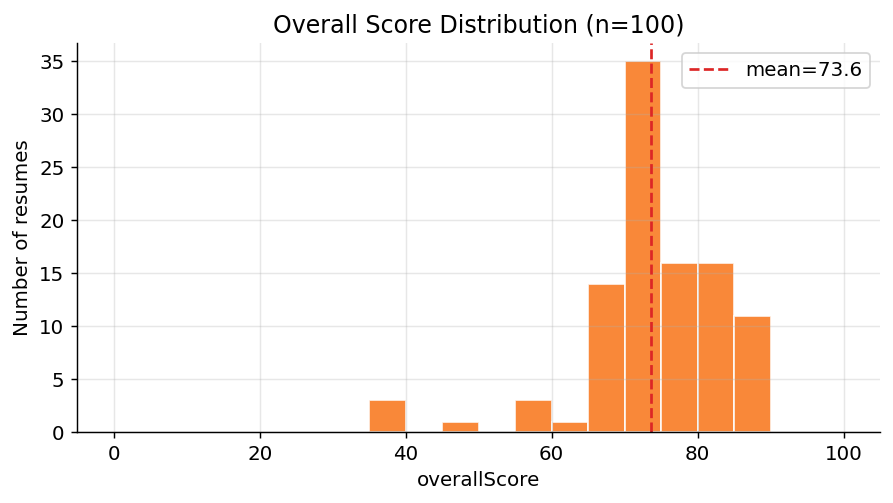
\includegraphics[width=0.86\textwidth]{figs/score_hist.png}
\caption{overallScore 评分分布}
\end{figure}

\begin{figure}[H]
\centering
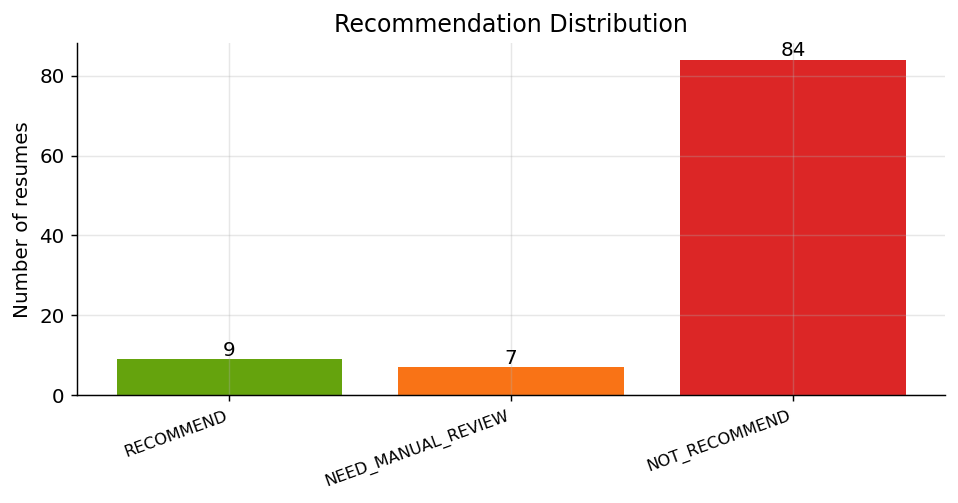
\includegraphics[width=0.86\textwidth]{figs/recommendation_bar.png}
\caption{推荐结论分布}
\end{figure}


\section{报告详细度（报告正文长度 / 面试追问条数）}
面试追问条数：均值 9.0，p50=10.0，max=10.0；
\textbf{追问 $\geq$ 8 的占比 87.0\%（87/100）}，验证报告详细度。
报告正文长度均值 154.8 字符。

\begin{figure}[H]
\centering
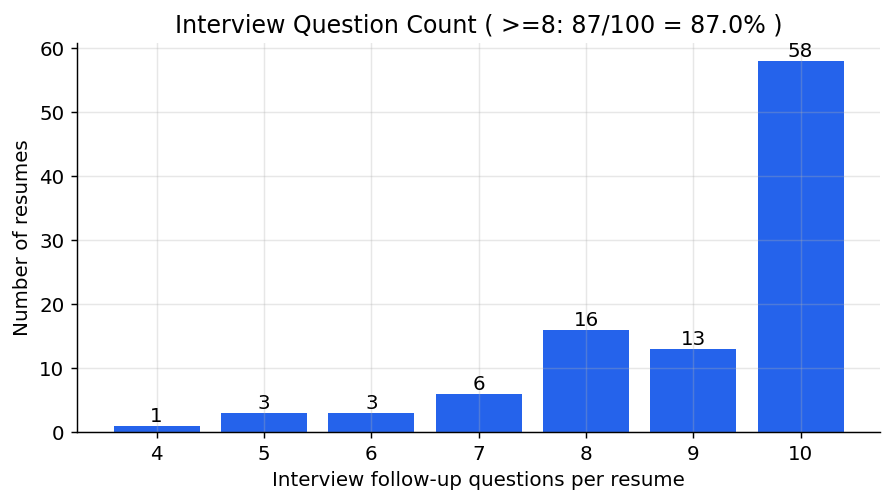
\includegraphics[width=0.86\textwidth]{figs/interview_hist.png}
\caption{面试追问条数分布}
\end{figure}

\begin{figure}[H]
\centering
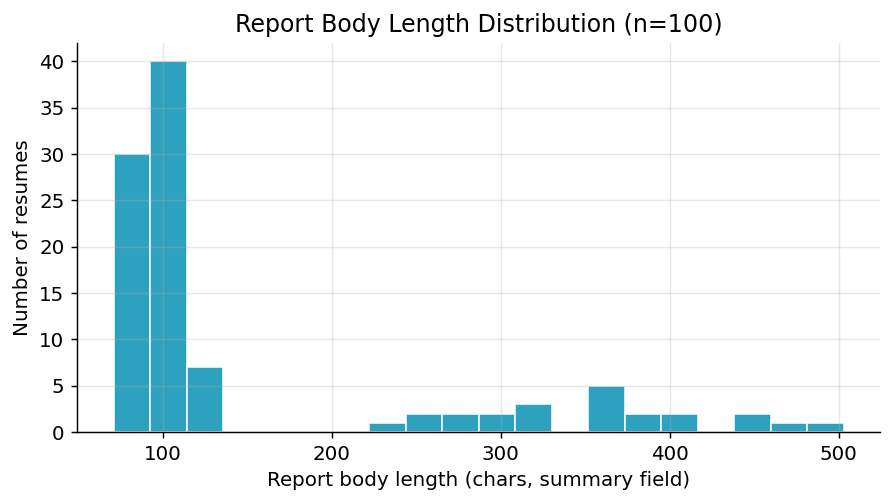
\includegraphics[width=0.86\textwidth]{figs/report_length_hist.png}
\caption{报告正文长度分布}
\end{figure}


\section{瓶颈分析与优化建议}
\begin{enumerate}[leftmargin=1.6em]
  \item \textbf{瓶颈节点：技术评估 TechEvalAgent（均值 13.86s）}。
  其包含一次 LLM 深度评估 + 向量批量检索 + （含外链时）github\_enrichment，是端到端时延主要来源。
  建议：对 \texttt{milvus\_resume\_batch\_search} 的多 query 并行化、对 LLM 评估启用更激进的 fast-lane 阈值、
  缓存高频 rubric 检索结果。
  \item \textbf{公网 MCP fetch 平均 3.15s}（p90 3.88s）是外部不可控时延。
  建议：对同一外链做结果缓存、设置更紧的超时与并发抓取、失败快速降级（trace 已显式可观测，便于熔断）。
  \item \textbf{报告生成节点均值 11.93s}。已通过\textbf{并行报告生成}将 ReportAgent 从早期约 37s 降到当前量级；
  可进一步将各章节流式拼接、对确定性段落走模板而非 LLM。
  \item \textbf{并发与排队}：墙钟 p90（54.9s）高于处理 p90（48.5s）的部分来自排队，
  说明在 4 并发下后端仍有吞吐余量可挖，建议结合限流与批处理进一步压缩排队。
\end{enumerate}

\section{面试可讲的亮点}
\begin{itemize}[leftmargin=1.4em]
  \item \textbf{动态路由真正省了大模型调用}：4 种 routeMode 按简历自适应裁剪 DAG，
  100 份累计省下 93 次 LLM 调用（13.3\%），每份平均仅 6.07 次，不是 PPT 数字而是 trace 实测。
  \item \textbf{公网 MCP 真实接入}：通过官方 \texttt{mcp-server-fetch} 实抓候选人外部主页，平均 3.15s，
  且时延在 trace 中可观测，触发率 70.0\% 与外链简历比例 70.0\% 吻合，证明是按需真实调用。
  \item \textbf{并行报告生成}：ReportAgent 由早期约 37s 降至均值 11.93s 量级，端到端 p50 仅 38.5s。
  \item \textbf{全链路可观测}：每个节点 durationMs、每次 toolCall 的 name/status/durationMs、harnessPlan 决策依据均落库，
  可做瓶颈定位、成本核算与回归门禁（本压测即基于该 trace 契约）。
  \item \textbf{规模化稳健}：100/100 份成功（成功率 100.0\%），4 并发下 p95=51.3s，
  失败可断点续跑。
\end{itemize}

\section{失败汇总}
本次压测\textbf{无失败任务}，100 份简历端到端全部成功。


\section*{附录：产出物清单}
\begin{itemize}[leftmargin=1.4em]
  \item 采集脚本：\texttt{harness/run\_stress.py}（可复现、断点续跑）
  \item 分析脚本：\texttt{harness/analyze.py}；报告生成：\texttt{harness/make\_report.py}
  \item 原始结果：\texttt{reports/stress\_e2e/raw\_results.json}；汇总：\texttt{summary.json}
  \item 图表：\texttt{reports/stress\_e2e/figs/*.png}
  \item 本报告：\texttt{reports/stress\_e2e/stress\_report.tex / stress\_report.pdf}
\end{itemize}

\end{document}
